
The previous chapter introduced QRNNs and DRNNs as machine-learning-based
methods to perform remote sensing retrievals. The motivation for this was to
find a practical approach to combine the capabilities of modern deep neural
networks with the theoretically sound handling of uncertainties of conventional,
inverse-theory-based retrieval methods. To explore the validity and practicality
of the proposed methods, they have been applied to idealized scenarios and
multiple real-world retrieval applications. This section presents this work and
summarizes the main results.

\section{Handling retrieval uncertainty with neural networks}

The first of the appended papers, entitled \textit{A neural network approach to
estimating a posteriori distributions of Bayesian retrieval problems} and
published as \citet{pfreundschuh18}, proposes using  QRNNs for remote
sensing retrievals. The study was motivated by the shortcomings of the
retrieval methods that were available at the time of its writing. The Bayesian
framework provides a principled way of handling uncertainties in remote
sensing retrievals (see Sec.~\ref{sec:machine_learning:retrieval_problem}),
but the commonly used methods are computationally complex. While retrievals
based on neural networks were already common and often offered superior
performance in terms of computational cost as well as accuracy, the retrieval
uncertainties were typically neglected.

The aims of the study are two-fold: (1) to demonstrate the compatibility of
QRNNs with conventional Bayesian retrieval methods and (2) to demonstrate the
practicality of QRNNs by applying them to a real-world retrieval application.

An idealized but realistic retrieval scenario in which the full Bayesian
solution could be calculated to arbitrary precision was designed to demonstrate
the compatibility of QRNNs with conventional Bayesian retrieval methods. The
study applies QRNNs and Bayesian Monte Carlo Integration (BMCI), a commonly used
Bayesian retrieval method, to solve the retrieval and compares their solutions
to the true solution. BMCI calculates an approximate solution of the retrieval
problem using a database of observations and corresponding reference values.
This makes it similar in this regard to machine learning methods. The results
show that QRNNs work at least as well as BMCI in solving the retrieval problem,
given that both are based on a sufficiently large dataset. There is a clearer
advantage for QRNNs for smaller datasets, indicating that they cope better with
the curse of dimensionality.

This first result has two important implications. Firstly, it showed that QRNNs
can be used instead of BMCI and expected to work at least as good given the same
training data. Even if the advantage of neural networks over BMCI on the
considered dataset was marginal when sufficient training data is available, the
use of neural networks offers distinct advantages compared to BMCI. For one, the
time required to produce a neural network prediction is independent of the
training data size. At least for a naive implementation of BMCI this time scales
linearly with the size of the training database. This means that the amount data
that can be used by the method may be limited by operational processing
requirements. Besides that, because of the flexibility of QRNNs, they can be
easily extended to image or time-series data, which is not as simple for BMCI or
other Bayesian retrieval methods.

The second important implication of these results is that they show the
compatibility of probabilistic machine learning methods with Bayesian retrieval
methods. These results link the extensive theory on Bayesian retrievals
\citep{rodgers00, tarantola05} with machine-learning-based methods. In
particular, the correspondence between the training data of the neural network
and the a priori distribution of a Bayesian retrieval highlights their
importance for accurate quantification of retrieval uncertainties.


%Two experiments were performed in the study. The first one used an idealized
%retrieval scenario in which samples from the posterior distribution $p(y|x)$
%could be calculated using Markov Chain Monte Carlo (MCMC) methods. MCMC is
%generally too slow to be used in operational processing, but its ability to
%generate samples from the true posterior distribution makes it suitable to
%provide a reference solution against which QRNNs and another Bayesian retrieval
%method could be evaluated. A principal results from this experiment is shown
%Fig.~\ref{fig:contributions:cdfs_qrnn_bmci}. The plot displays the retrieved
%CDFs of the posterior distributions using QRNN and Bayesian Monte Carlo
%Integration (BMCI), which is a commonly used Bayesian retrieval methods. Each
%panel shows the reference CDF obtained using MCMC in the background and the CDFs
%obtained using BMCI in blue, those obtained from a single QRNN using a solid red
%line and those obtained from an ensemble of QRNNs using red markers. The shown
%samples were chosen according to the Kolmogorov-Smirnov of the BMCI
%($\text{KS}_\text{BMCI}$) and QRNN ($\text{KS}_\text{QRNN}$), which measures
%the agreement between the reference and retrieved CDF, and thus show retrieval
%results of varying quality from each retrieval.
%
%The main finding from this first experiment is that the CDFs retrieved using
%QRNN and BMCI agree very well with the reference CDF calculated using MCMC. This
%indicates that probabilistic neural network retrievals are consistent with the
%Bayesian solution of inverse problems with the a priori distribution being
%represented by the training data.
%
%\begin{figure}
%  \centering
%  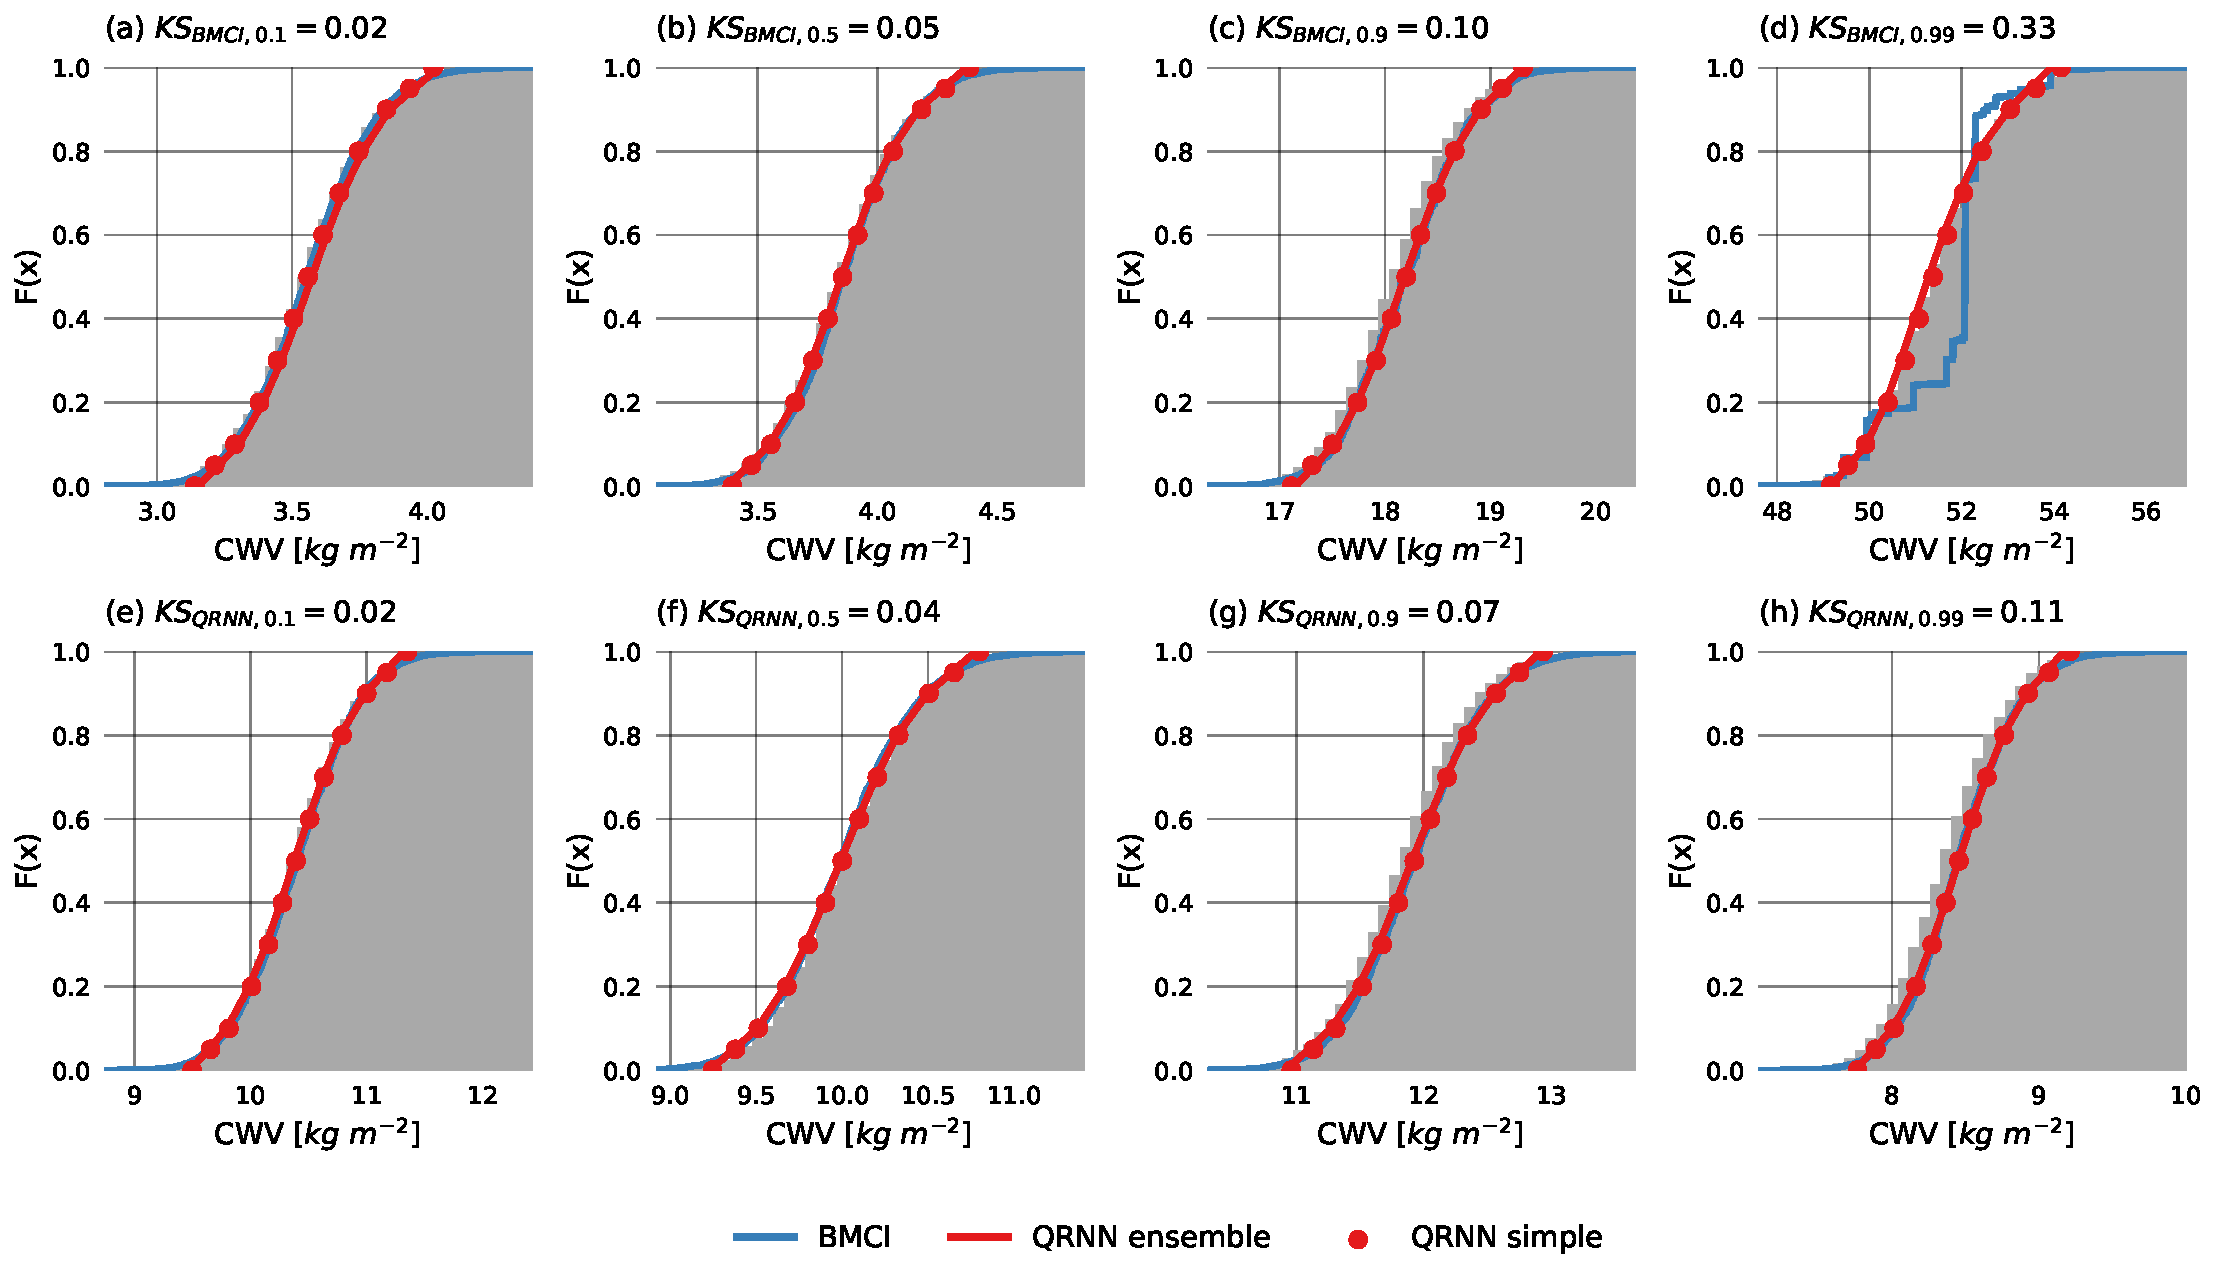
\includegraphics[width=\textwidth]{cdfs_qrnn_bmci}
%  \caption{ Retrieved a posteriori CDFs obtained using MCMC (gray), BMCI (blue),
%    a single QRNN (red line) and an ensemble of QRNNs (red marker). Cases
%    displayed in the first row correspond to the 1st, 50th, 90th and 99th
%    percentiles of the distribution of the Kolmogorov– Smirnov statistic of BMCI
%    compared to the MCMC reference. The second row displays the same percentiles
%    of the distribution of the Kolmogorov–Smirnov statistic of the single-QRNN
%    predictions compared to MCMC.}
%  \label{fig:contributions:cdfs_qrnn_bmci}
%\end{figure}

The second experiment from this study applied QRNNs to the retrieval of cloud
top pressure (CTP) from infrared observations from the Moderate Resolution
Imaging Spectroradiometer (MODIS). The comparison of the QRNN retrieval to an
existing algorithm based on a deterministic neural network shows that QRNNs
yield comparable or better accuracy for point predictions with the added benefit
of providing reliable uncertainty estimates.

A principal result from this experiment is shown in
Fig.~\ref{fig:contributions:qrnn_errors}, which shows the predicted and observed
distributions of retrieval errors for QRNNs as well as for the deterministic
retrieval combined with a Gaussian error model fitted on the test data. As the
comparison of the distribution shows, the Gaussian error model does not provide
a good description of the retrieval error, whereas the QRNN successfully
predicts its distribution. This results shows the ability of the QRNN to
represent non-Gaussian retrieval errors and the superiority over commonly
assumed Gaussian error models. A consequence of these findings was the adoption
of QRNNs for the operational production of near-real-time retrievals of cloud
top pressure at the European Organisation for the Exploitation of Meteorological
Satellites.

\begin{figure}
  \centering
  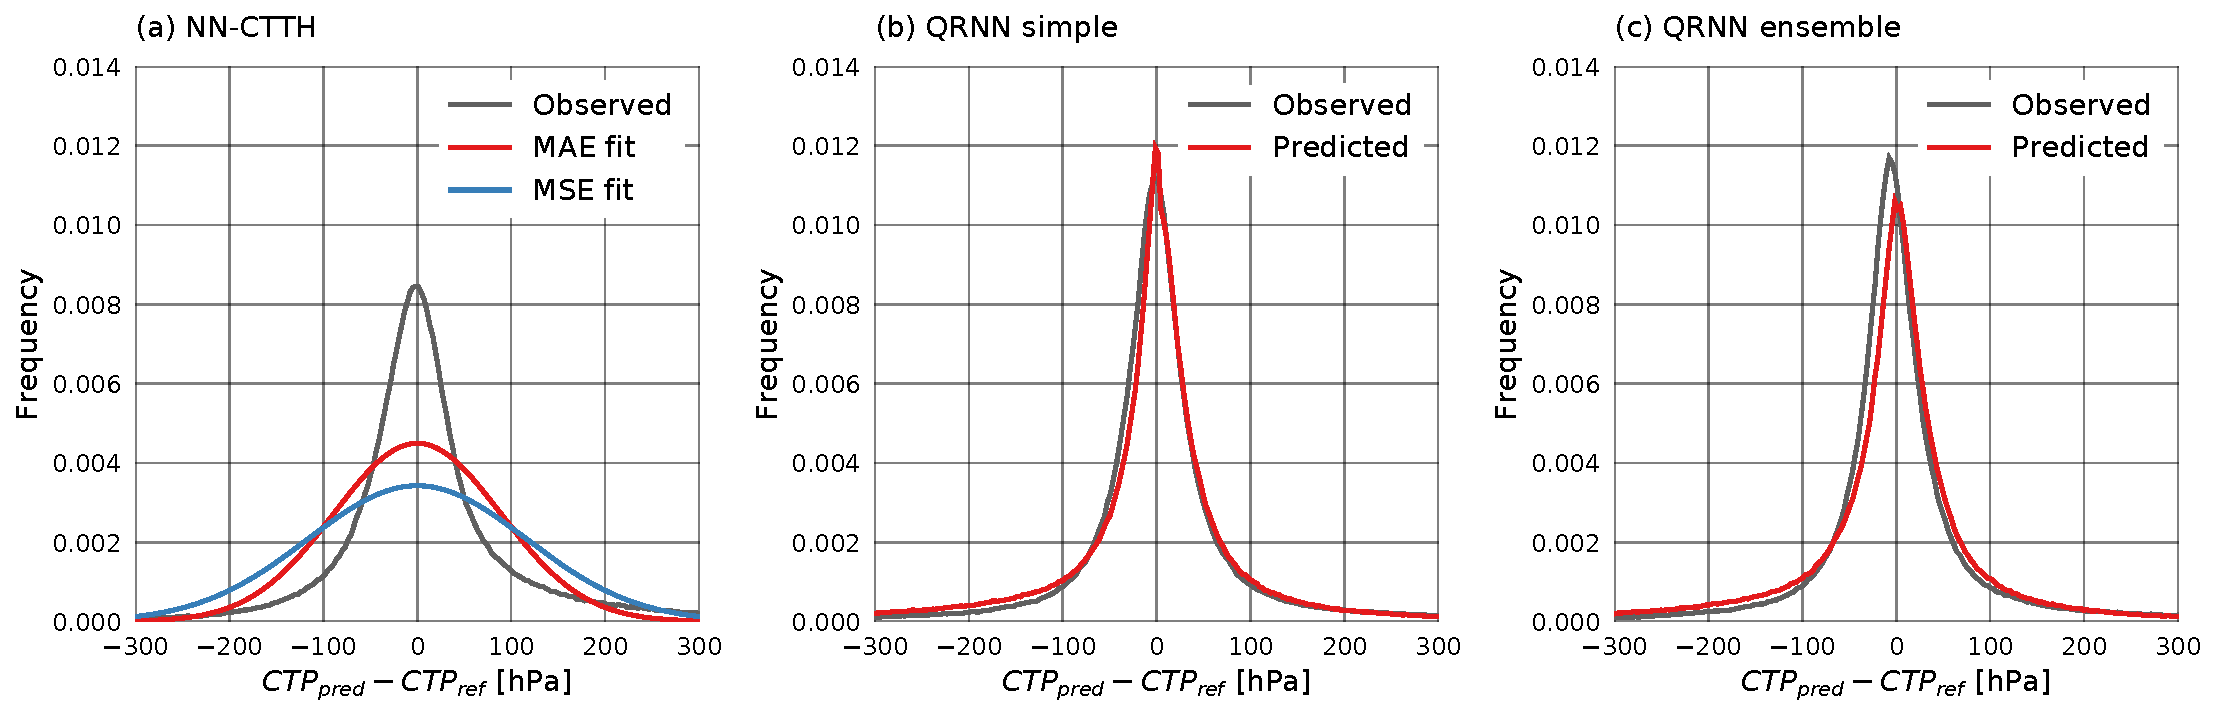
\includegraphics[width=0.75\textwidth]{qrnn_predicted_errors}
  \caption{Distributions of predicted and observed cloud-top pressure (CTP)
    retrieval errors. Panel (a) shows the results for a deterministic neural
    network combined with a Gaussian error models fitted used the mean squared
    error (blue) and the mean absolute error. Panel (b) show the
    corresponding results for the QRNN retrieval.}
  \label{fig:contributions:qrnn_errors}
\end{figure}

\section{Passive microwave precipitation retrievals}

The second study included in this thesis, entitled \textit{ GPROF-NN: A neural
  network based implementation of the Goddard Profiling Algorithm} and published
as \citet{pfreundschuh22a}, applied the QRNN methodology to the retrieval of
precipitation from passive microwave (PMW) observations of the GPM mission (see
Sec.\ref{sec:radiative_transfer:synergies}). GPM is an international satellite
mission lead by NASA and JAXA, which aims to provide global measurements of
precipitation at high spatial and temporal resolution.

 %The mission is built around the Core Observatory satellite, which carries a
 % precipitation radar and a PMW sensor dedicated to the remote sensing of
 % precipitation. Retrievals from the combined radar/PMW observations from the
 % Core Observatory are used to build a retrieval database that is in turn used
 % to for the retrievals of a constellation PMW sensors. As of this writing, the
 % GPM constellation comprises 9 active satellites.

The algorithm that is used to retrieve precipitation from GMI, the PMW
sensor on the GPM core observatory, and the other PMW sensors of the GPM
constellation is the Goddard Profiling Algorithm (GPROF,
\citeauthor{kummerow15}, \citeyear{kummerow15}). GPROF is based on the BMCI
method and retrieves surface precipitation as well as profiles of hydrometeor
concentrations and latent heating rates. The aim of the study was to assess the
potential benefits of replacing BMCI with a neural-network-based retrieval.
Besides that, it aims to explore to what extent the accuracy can be improved if
spatial information is incorporated into the retrieval instead of processing
each pixel separately as the current implementation does. To this end, two
neural-network-based implementations were developed. The first one, named
GPROF-NN 1D, uses an MLP to retrieve precipitation from a single pixel. The
second one, GPROF-NN 3D, uses a CNN to retrieve precipitation using  the full
swath of observations. This allows the GPROF-NN 3D retrieval to leverage
structural information in the observations, which is not available to the two
other implementations.

Both the GPROF-NN 1D and GPROF-NN 3D retrieval were developed to be functionally
equivalent to the currently operational GPROF algorithm so that they can
potentially replace it in an upcoming update. Moreover, the implementations were
restricted to use exactly the same data for their training as the current
method, which was done to ensure that the comparison of the three methods isn't
obscured by differences in the training data.

While the application of QRNNs to the GPROF algorithm is in principle
straightforward, the requirement to develop a retrieval that uses and produces
identical in- and output data and is based on the same data as the current
implementation of GPROF proved challenging. The training data for the sensors of
the GPM constellation makes use of radiative transfer simulations. However,
these are not generated for full swaths of observations but only for single
pixels. This makes the simulation data unsuitable for the training of CNNs.
Since extending the simulations to the full swath is currently not possible, an
intermediate CNN-based `retrieval' was trained to emulate the simulations of PMW
observations.

%proved challenging especially for the GPROF-NN 3D retrieval. The training data
%for all sensors of the GPM constellation is based on combined radar/radiometer
%observations from the GPM satellite. Since these observations are only available
%at a $\SI{100}{\kilo \meter}$-wide swath at the center of the GMI observations,
%a way had to be found to extent these to the full GMI-swath and to remap them to
%the viewing geometries of the other sensors. The current approach uses an
%intermediate simulator network to extend the simulated observations to the full
%swath of GMI, which are then remapped to the viewing geometries of other sensors
%by interpolation. This solution should be a considered a heuristic that was
%pursued mainly because extending the simulations that are routinely performed
%for the generation of the GPROF training data would have been outside the scope
%of this study.

The main results from this study are estimates of potential improvements in
retrieval accuracy that are achievable by upgrading GPROF to either the GPROF-NN
1D or GPROF-NN 3D retrieval. Consistent improvements for the GPROF-NN 1D
algorithms are found across a range of accuracy metrics for the retrieved
surface precipitation as well as the hydrometeor profiles. The accuracy is
improved further by the GPROF-NN 3D retrieval, which yields improvements similar
in magnitude to those provided by the GPROF-NN 1D algorithm over the GPROF
baseline retrieval. Furthremore, we found that the effective resolution of the
retrieval improves by at least $\SI{40}{\percent}$ for the neural-network-based
retrievals.

An example of the improvements afforded by the neural-network-based retrievals
is shown in Fig.~\ref{fig:machine_learning:hurricane_harvey}. This plot shows
the smoothed surface precipitation from the combined retrieval from the GPM core
observatory as a reference and the retrievals from the GPROF and GPROF-NN
algorithms. The comparison shows that the GPROF-NN retrievals are spatially
better resolved and improve the agreement with the combined retrievals.

\begin{figure}
  \centering
  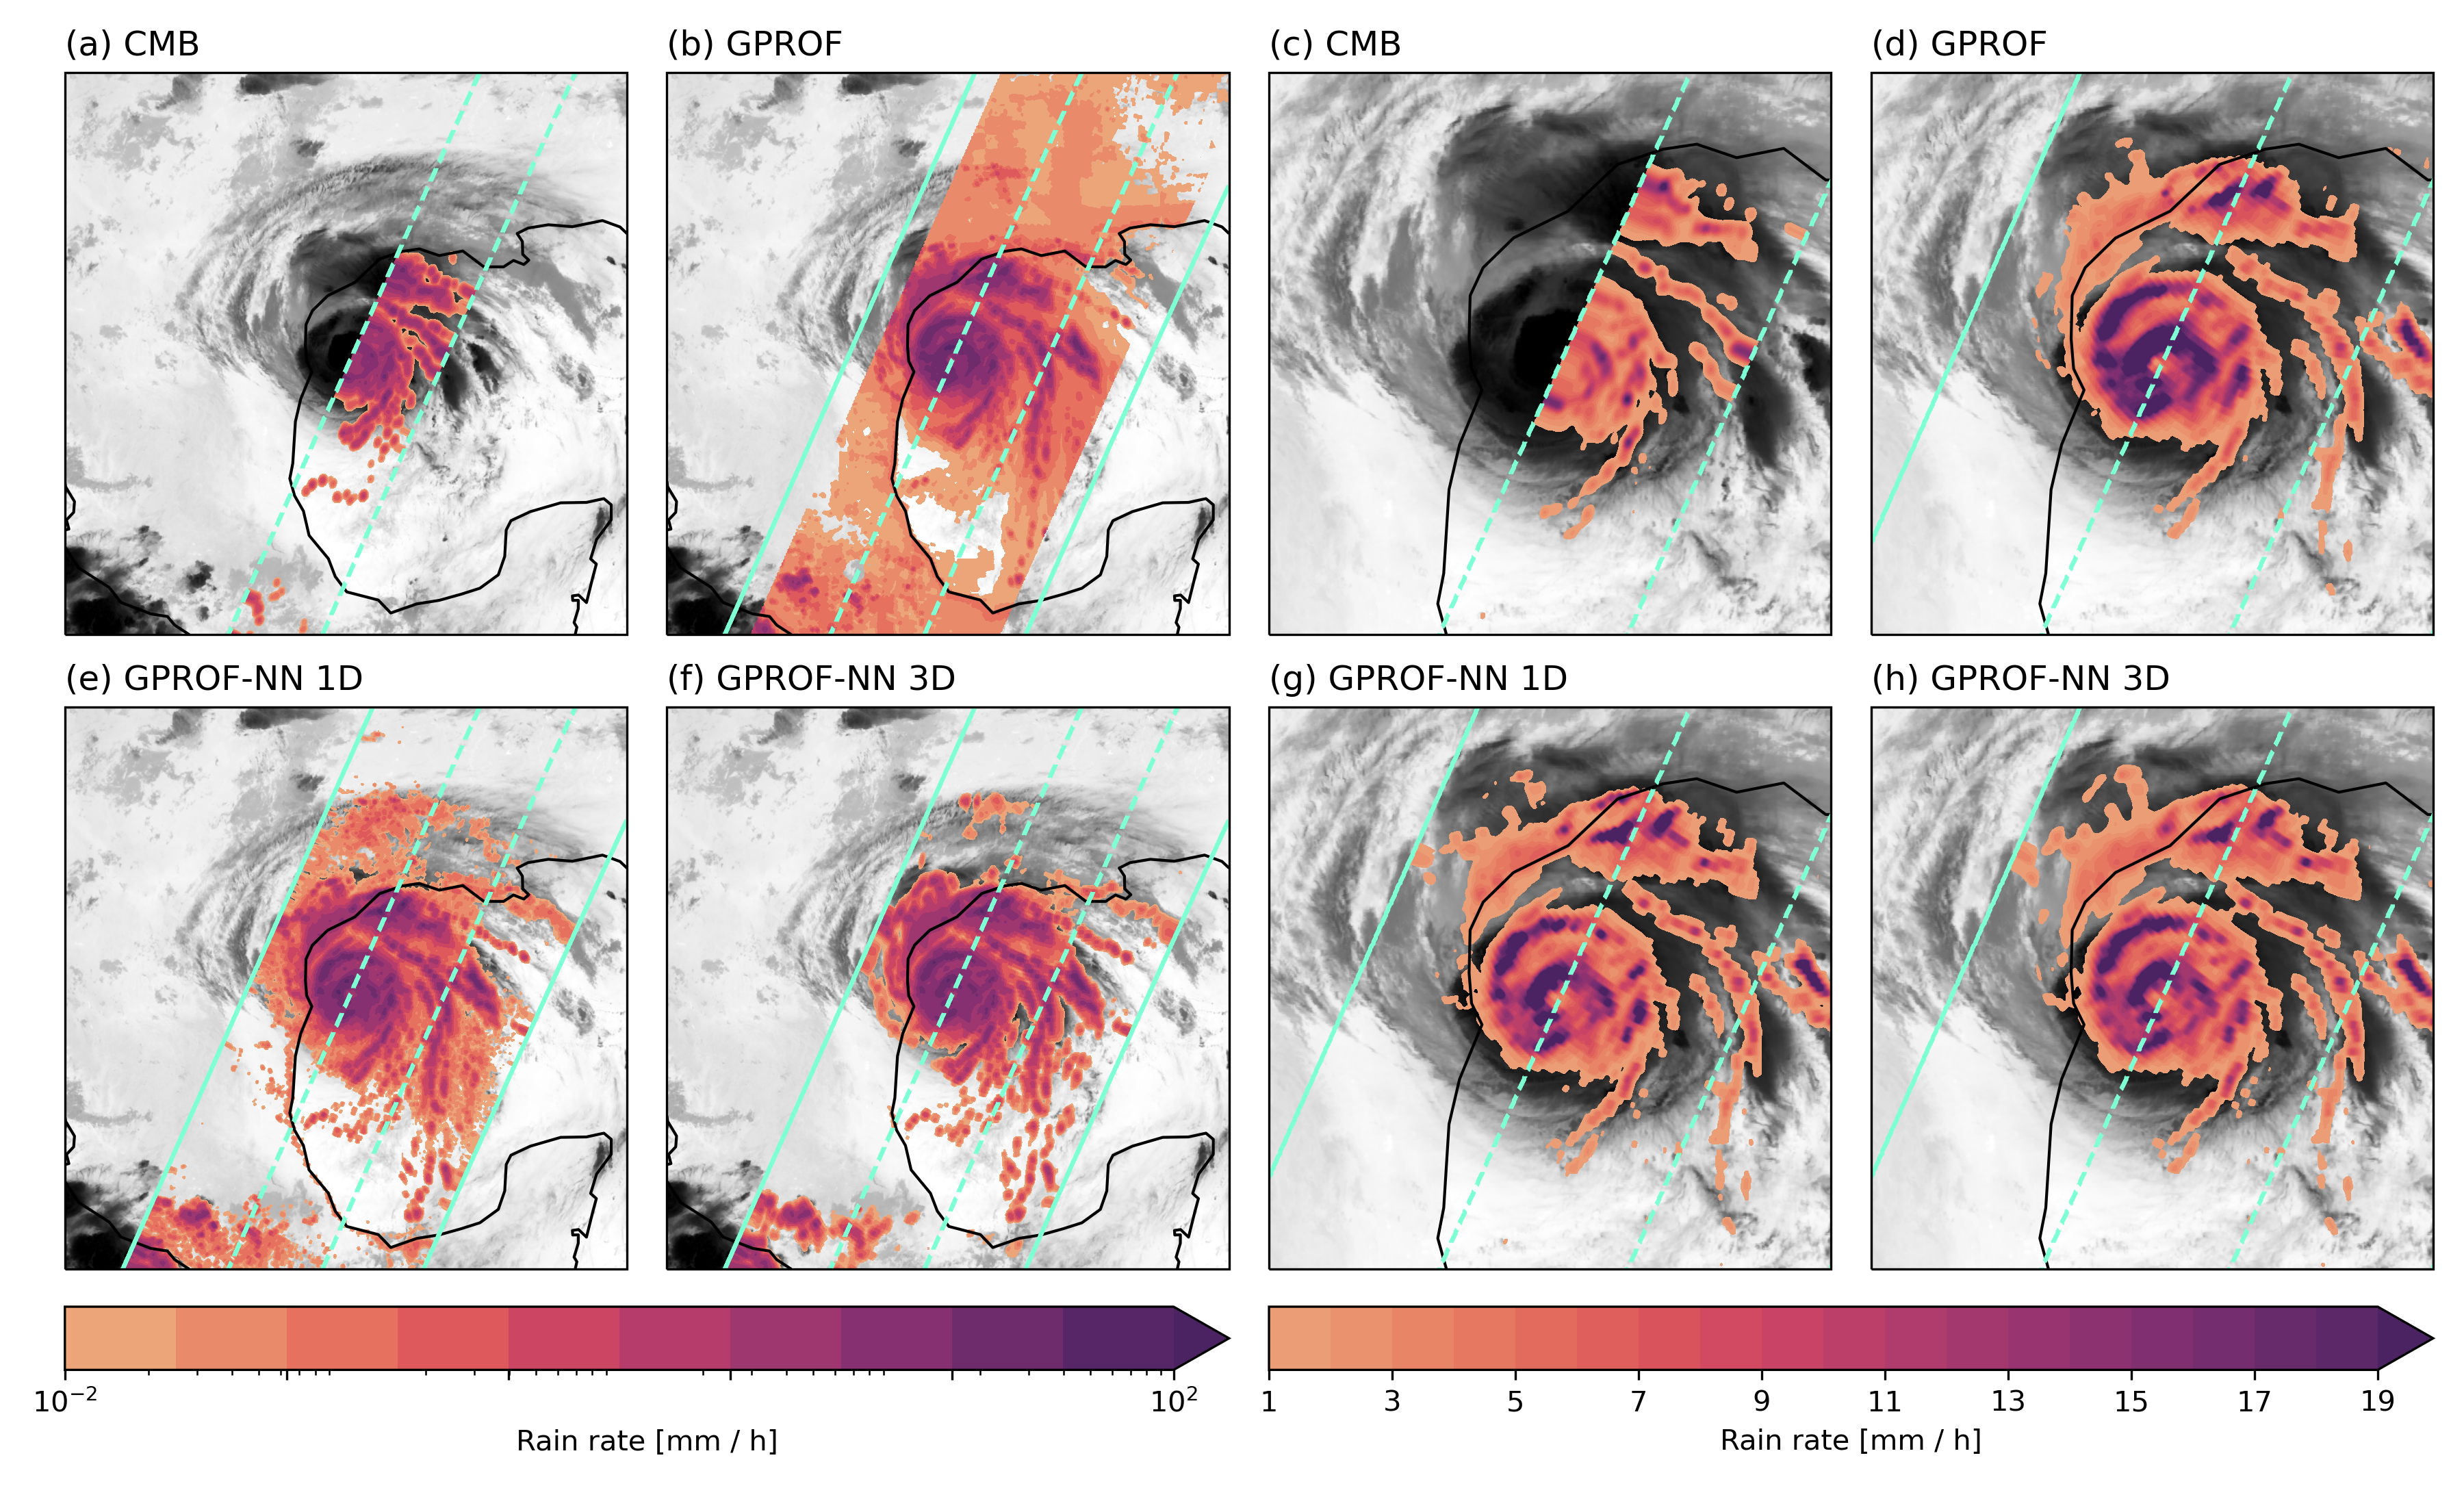
\includegraphics[width=\textwidth]{surface_precip_harvey_gmi_ir}
  \caption{ Retrieved surface precipitation from the GPM combined product
    (Panels (a), (c)), the GPROF algorithm (Panels (b), (d)), and the neural
    network versions GPROF-NN 1D (Panels (e), (g)) and GPROF-NN 3D (Panels (f),
    (h)) in and around Hurricane Harvey on 2017-08-25 at 11:50:00 UTC. Panels
    (a), (b), (e), (f) display the precipitation on a logarithmic scale over an
    area spanning $2\ 000\ \unit{km}$ in zonal and meridional directions.
    Panels (c), (d), (g), (f) display the surface precipitation on a linear
    color scale in an enlarged area spanning $500\ \unit{km}$ around the
    Hurricane. The background shows $10.3\ \unit{\mu m}$ brightness temperatures
    from the GOES 16 observations closest to the overpass.
  }
  \label{fig:machine_learning:hurricane_harvey}
\end{figure}

Although the results from this study were promising, their significance was
limited because the evaluation of the retrieval was restricted to the same
source of data that was used for the generation of the training data. Since the
objective of the study was to compare the BMCI retrieval method with QRNNs, this
simplification was justified. In a validation against independent data,
potential benefits may be obscured by deviations between training data and the
data used for validation. However, the practically more relevant question is, of
course, to what extent the neural network retrievals improve the precipitation
estimates when compared to independent validation data.

A study that addresses this question is currently under preparation and included
in this thesis as the third paper, entitled \textit{%
  Evolution of the GPROF
  passive microwave precipitation retrievals evaluated against ground radar
  measurements over the continental US and the Pacific Ocean%
}. Since the
  development of the GPROF-NN algorithms was performed in parallel with a new
  version of the GPROF retrieval, this study aimed to assess improvements in
  this new version of GPROF (GPROF V7) against the previous version (GPROF V5)
  , as well as the potential benefits of replacing GPROF with GPROF-NN 1D or 3D in
  a future update. Furthermore, the study aims to identify potential outstanding
  issues impeding the adaptation of the GPROF-NN retrievals for operational
  processing.

The validation is based on ground-radar measurements of precipitation
specifically created for the validation of GPM measurements. It is
based on measurements from the continental United States (CONUS) and a ground radar
station on the Kwajalein atoll in the Pacific Ocean.

The main focus of this study is put on retrievals from the GMI radiometer, which
plays a special role in the GPM constellation due to it being designed
specifically for the remote sensing of precipitation. The accuracy of the
precipitation retrieved from the GMI sensor using the two versions of the
conventional GPROF algorithm as well as the two GPROF-NN retrievals is evaluated
for two years of co-locations. The results clearly show that the benefits of the
neural-network-based implementation of GPROF carry over to validation against
independent precipitation measurements. In particular, the effective resolution
of the retrieved precipitation over land is improved  by more than a
factor of two.

The principal results from this study are shown in
Fig.~\ref{fig:machine_learning:gprof_nn_metrics}. The graphs show error metrics
of the retrieval when compared against the training data (labeled Database) as
well as compared against ground-based radar measurements over the period of two
years. These results clearly show that the GPROF-NN retrievals consistently
improve the instantaneous errors in the retrieval. For the biases,
the results are less obvious, but the fact that the combined retrieval
(labeled GPM-CMB) exhibits similar biases suggests that the origin for these
biases is at least in part in the training data itself.

  \begin{figure}[!hbpt]
    \centering
    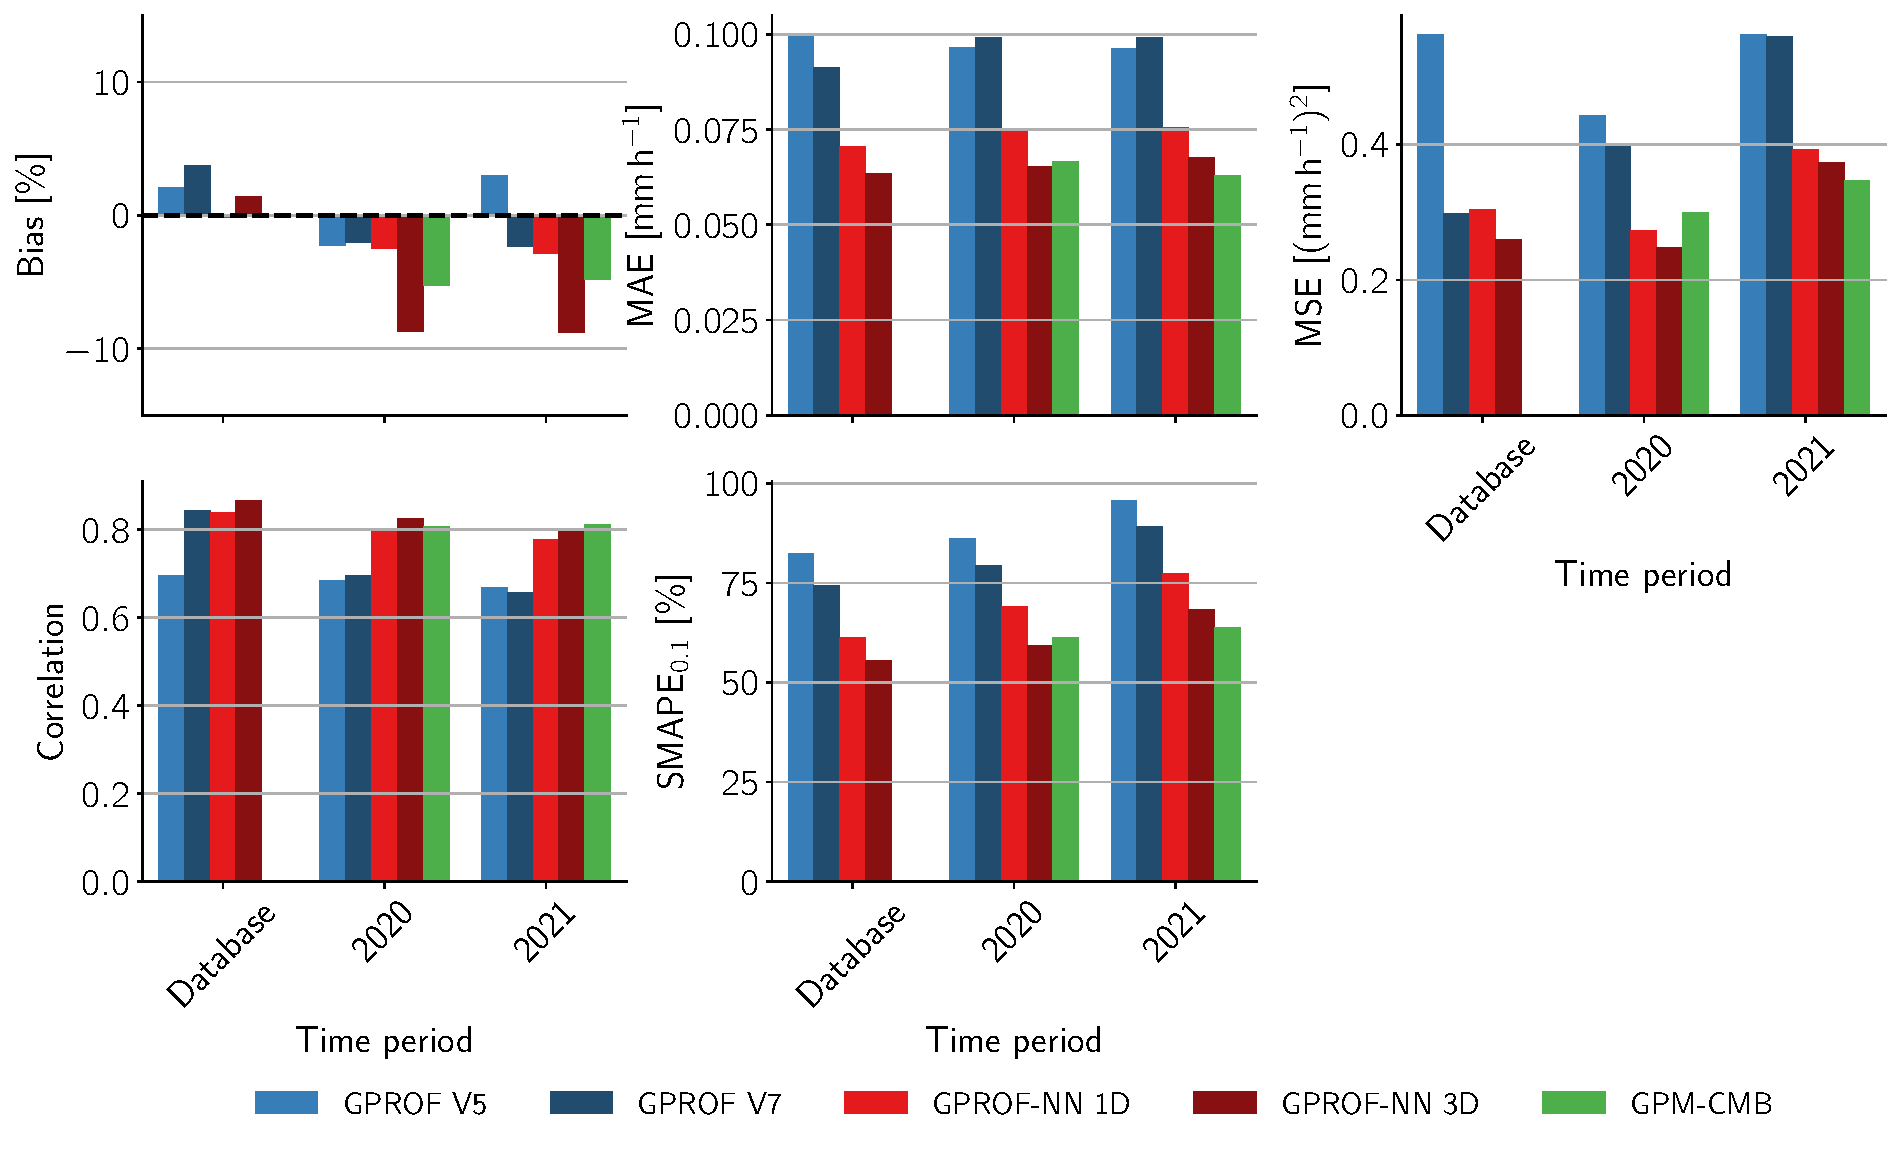
\includegraphics[width=\textwidth]{gprof_nn_metrics.pdf}
    \caption{
      Accuracy metrics of the GPROF retrievals compared to the training data
      (Database) and gauge-corrected ground-radar measurements for the water
      years 2020 and 2021.
    }
    \label{fig:machine_learning:gprof_nn_metrics}
  \end{figure}

In addition to GMI, also the retrieval accuracy of a limited number of other
sensors of the GPM constellation is evaluated. For the two sensors that have
been evaluated so far, smaller improvements in retrieval accuracy are found.
This is nonetheless an encouraging result because these sensors is affected by
errors in the radiative transfer simulation required to generate the training
data, which is not the case for the retrieval for GMI.

\section{Near real-time rain retrievals over Brazil}

While the neural-network-based implementation of GPROF provided  evidence
for the potential of neural-network-based precipitation retrievals, the
constraint of a retrieval that provides the same output as the current
operational GPROF algorithm did not leave much room to explore retrieval
improvements afforded by the probabilistic retrieval results. The two studies on
the development and assessment of the GPROF-NN retrievals presented above
therefore focused mostly on deterministic precipitation estimates and did not
explore the full potential of the probabilistic predictions afforded by the
neural networks.

The aim of the third study presented in this thesis, titled \textit{%
  An
  improved near real-time precipitation retrieval for Brazil%
} and published as
  \citet{pfreundschuh22b}, was to explore the full potential of probabilistic
  neural-network based precipitation retrievals in the context of near real-time
  retrievals from VIS and IR observations over Brazil. The input data for the
  retrieval comes from the advanced baseline imager (ABI, \citeauthor{schmit18},
  \citeyear{schmit18}) on the geostationary operational environmental satellite
  (GOES) 16. The input observations were co-located with
  retrievals from the combined radar and passive microwave observations
  from the GPM Core Observatory to generate the training data.

%The disadvantage of the observations of the ABI for precipitation retrievals is
%that they are limited to the VIS and IR regions and therefore only provide only
%indirect information on surface precipitation. However, their ability to provide
%observations every $\SI{10}{\minute}$ over Brazil and their very high spatial
%resolution still justifies their application for precipitation near real-time
%precipitation retrievals.

To validate the neural-network-based retrievals, their results were compared to
one month of gauge measurements. The retrieval accuracy was assessed by
comparing it to the retrieval algorithm that is currently used operationally at
the Brazilian National Institute of Space Research as well as two other
commonly used, global precipitation retrievals. This comparison shows that,
despite the limited information content of VIS/IR observations,
deep-learning-based retrievals outperform currently available methods, even
those that merge IR observations from geostationary satellites with passive
microwave observations.

Assessment of the predicted uncertainties against the gauge measurements shows
that they are reliable, given that differences between training  and reference
 data are taken into account. In addition to that, the study presented ways
of leveraging probabilistic retrieval results to improve the characterization of
precipitation. The predicted uncertainties can be used, for example, to derive
the probability of the observed rain exceeding a given threshold. When the
probabilistic prediction are used in this way, the retrieval  outperforms
all reference retrievals for the detection of heavy precipitation events.
Moreover, when the predicted distributions are used to generate samples from the
a posteriori distribution of the retrieval, the agreement between the
distributions of retrieved and gauge-measured precipitation is improved.
Including these samples in the retrieval output thus provides a way of improving
the representation of precipitation extremes in the retrieval results.

Fig.~\ref{fig:contributions:hydronn_case_study} shows the results of the reference retrievals
as well as the Hydronn neural-network-based precipitation retrievals that were
developed in this study. The results correspond to a flood-producing
precipitation event that occurred during the evaluation period. Each panel shows
the results for one or more retrievals together with the reference gauge
measurement. Panel (a) shows the results for the assessed reference retrievals.
Only one of them predicts significant precipitation during the event. Panels
(b), (c), and (d) show the corresponding results for the three configurations of
the Hydronn retrieval with the predicted mean precipitation shown by the solid
line and the shading showing the posterior CDF at quantile fractions $[0.01,
  0.1, 0.2, \ldots, 0.8, 0.9, 0.99]$. Although the predicted mean precipitation
is as low as that of the best reference retrieval, the spread in the
uncertainties clearly shows the risk of much higher precipitation.

\begin{figure}
  \centering
  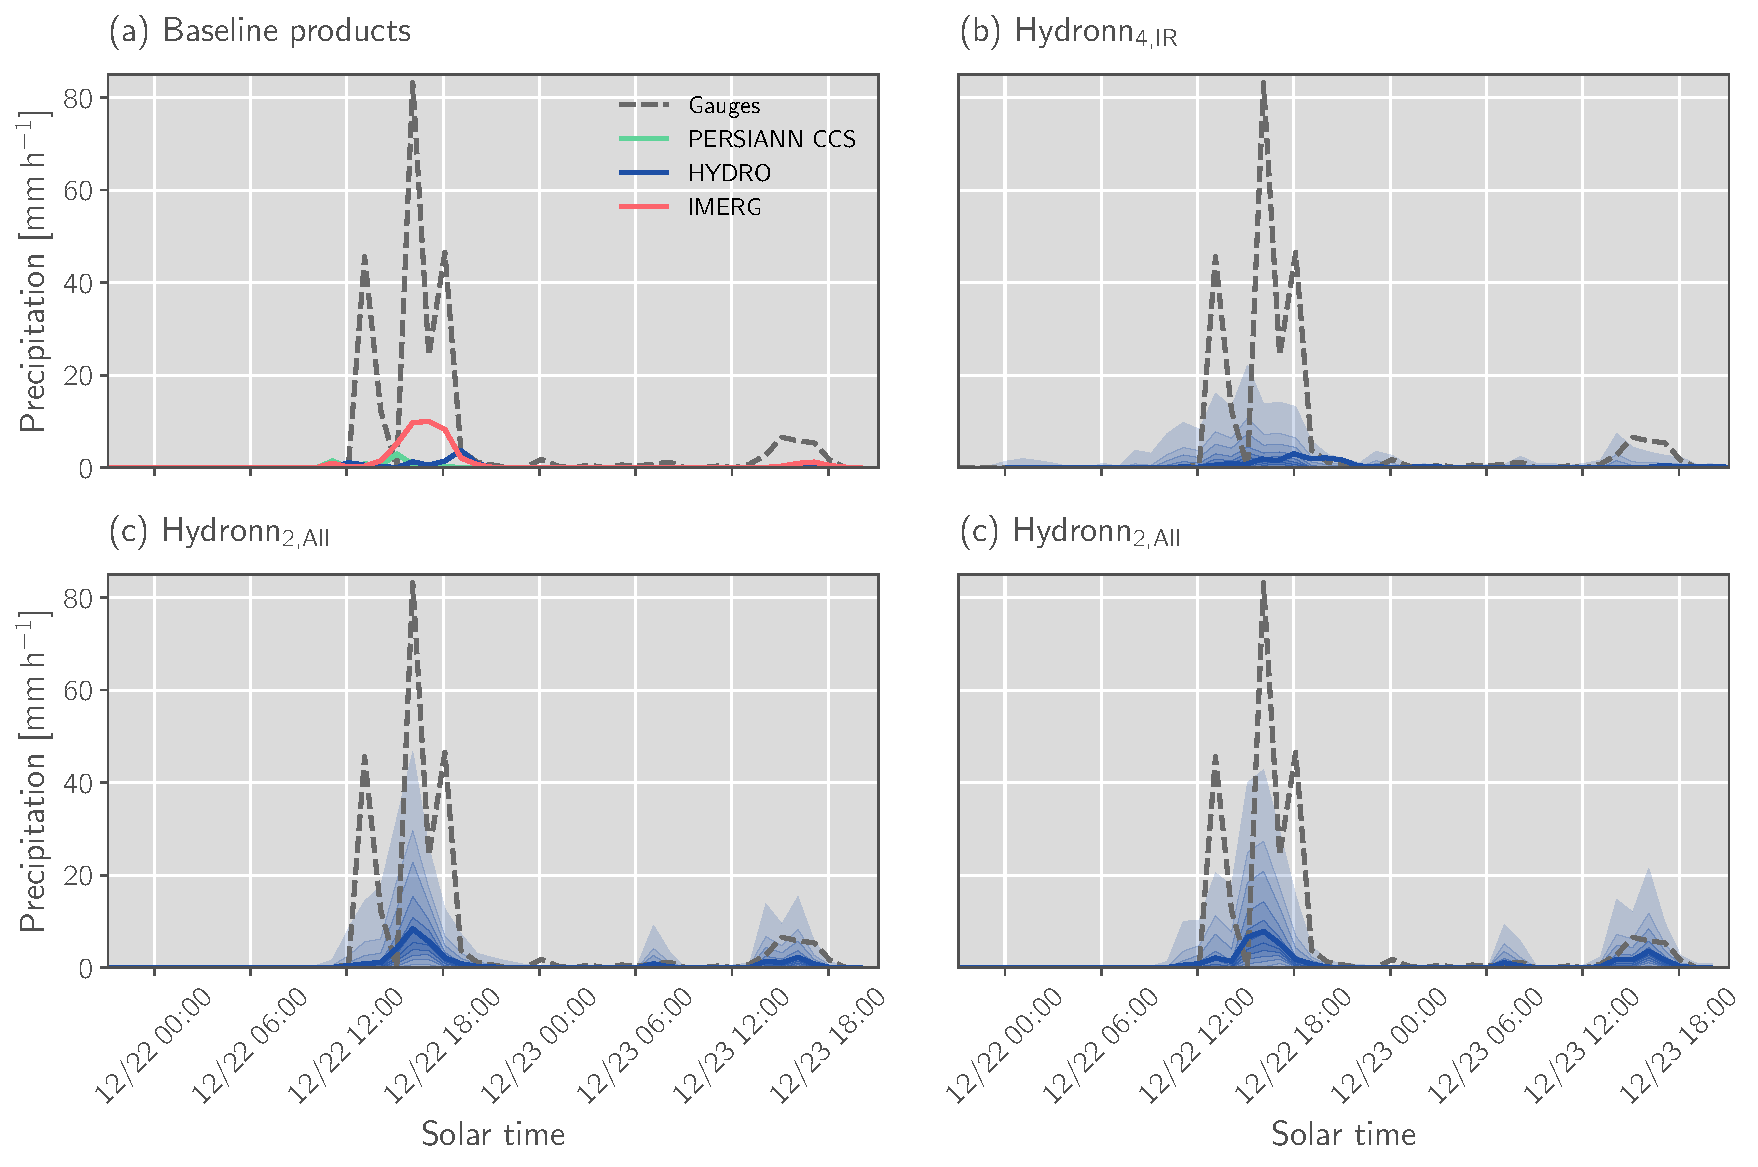
\includegraphics[width=\textwidth]{hydronn_case_study}
  \caption{
      Retrieved precipitation for a flood-producing precipitation even that
      occurred between 2020-12-22 and 2020-12-24 in the cite of Duque de Caxias
      in the state of Rio de Janeiro. Grey, dashed lines show the precipitation
      by the gauge station in Xer\'em. Solid lines show the retrieved mean
      precipitation for each retrieval algorithm. The shading shows filled
      contours of the posterior CDF at values $[0.01, 0.1, 0.2, \ldots, 0.8,
        0.9, 0.99]$.
    }
  \label{fig:contributions:hydronn_case_study}
\end{figure}

Besides a significantly improved near real-time retrieval for application over
Brazil, the principal results from this study are further proof of the ability
of neural-network-based retrievals to leverage the full potential of
latest-generation satellite imagery. The configuration that uses all available
channels at the highest possible resolution outperforms the GPM IMERG product,
which is one of the most advanced precipitation retrievals currently available
and integrates observations from a wide range of sensors and gauge measurements.

However, as can be seen in the results in
Fig.~\ref{fig:contributions:hydronn_case_study}, the retrievals from VIS and IR
observations still remain limited in their capabilities of detecting extreme
precipitation. While deep neural networks yield significant improvements in
retrieval performance, their instantaneous accuracy will always be limited by
the low information content of the observations. This suggest that future
retrieval development should try to further increase the amount of information
available to the retrieval, for example by incorporating the temporal evolution
of the observations or by merging observations from multiple sensors types.

\section{Cloud correction for data assimilation}

The final study included in this thesis is entitled
\textit{
  Can machine learning correct microwave humidity radiances for the influence of clouds?
  }
and published as \citet{kaur21} explores the application of QRNNs to remove the
effect of clouds from microwave observations. These observations contain
information on the temperature and distribution of water vapor in the atmosphere
and are used in data assimilation systems to find good initial conditions for
numerical weather forecasts. Since the assimilation usually involves simulating
the observations, the presence of hydrometeors in the atmosphere makes the
handling of observations that are affected by clouds much more complex. The
assimilation of both cloud-free and cloudy observations is referred to
as \textit{all-sky} assimilation. However, due to the complexity of handling the effects
of hydrometeors, less advanced assimilation systems discard cloudy observations
and only assimilate clear-sky observations.

This study investigates whether QRNNs can be used to detect and remove the
effect of clouds on microwave observations. If a model existed that could
accurately predict how cloudy-sky observations would look when the effect of
hydrometeors is removed, then this could, in principle, be used to handle these
observations in clear-sky assimilation systems. Since the ability to handle
cloud-affected observations significantly increases the number of observations
that can be ingested by the system, such a model could thus help to improve the
initialization of weather forecasts.

Because of their impact on the radiative transfer, operational data assimilation
systems have to detect observations affected by hydrometeors to either inflate
the uncertainties assigned to the observations (for all-sky assimilation) or
discard them altogether. Therefore, the first experiment in this study  assesses
the potential of applying QRNNs to predict a correction for cloud-contaminated
observations using an existing satellite sensor and compares the performance to
existing methods. The experiment shows that the QRNN-derived correction leads to
a lower bias in the observations than the residual biases in currently used
filtering methods, which reject up to $\SI{30}{\percent}$ of the observations.

The second experiment extended the approach to an upcoming satellite that will
be launched soon and a concept for a future satellite. Both of these satellites
will carry microwave sensors with channels above $\SI{300}{\giga \hertz}$. These
high frequencies make the observations more sensitive to scattering from ice
particles, which further complicates their use in data assimilation. In these
cases, using a QRNN-based cloud correction would provide a way to use the
additional information from the high-frequency channels to provide a more
accurate correction of lower frequency observations, which would improve the
impact of the lower frequency observations in the assimilation system. The
results show that observations at frequencies exceeding $\SI{300}{\giga \hertz}$
are well suited for cloud correction and thus demonstrate the potential of this
approach.

The principal result from this study is a proposed novel application of QRNNs
for the correction of microwave observations for use in data assimilation.
QRNN-based cloud correction provides superior performance to existing methods,
and the predicted uncertainties are more accurate than error estimates from
currently used error models. Moreover, the simulation-based assessment of the
potential of microwave observations at sub-millimeter wavelengths led to the
selection of these channels for an upcoming satellite mission
\citep{arctic_weather_satellite}.

\section{Future work}

The findings of this thesis suggest several directions of future research.
These will be discussed below.

\subsection{Handling retrieval uncertainty with neural networks}

This thesis has proposed and assessed neural-network-based methods for handling
uncertainties in remote sensing retrievals and shown their practicality across
multiple retrieval applications. The principal advantage of these methods is
certainly their simplicity. A minor modification in the training process is
required to migrate a deterministic neural network retrieval to a probabilistic
one. There are, however, two important limitations of the approaches: Their
incapability to handle correlations in the retrieval outputs and their reliance
on the aleatoric assumption, which postulates that the predictive uncertainty is
dominated by the aleatoric uncertainty.

It would therefore be valuable to systematically evaluate the approaches against
Bayesian neural networks and generative models on a set of atmospheric retrieval
problems. Such an evaluation should assess not only the retrieval accuracy but
also to take into account the effect on downstream applications of the data.
This would provide guidance in what scenarios the computationally more complex
alternative approaches should be applied.

\subsection{GPM precipitation retrievals}

Due to the good performance of the developed GPROF-NN retrievals, they are being
considered for the operational processing of the passive microwave retrievals of
the GPM mission. This will require additional investigations regarding the
climatological stability of the GPROF-NN retrievals across different satellites.

In addition to that, the migration to a neural-network-based implementation
opens up a number of opportunities for further improvements of the GPM passive
microwave retrievals. One of them is the extension of the training data to cover
multiple years of observations. It was found in \citep{pfreundschuh22d} that the
limited training period may be one reason for the retrieval errors on
climatological time scales. Besides that, including samples from the posterior
distribution may improve the representation of extreme precipitation in the
retrieval results, which is highly relevant for climate change studies.

\subsubsection{Novel retrieval applications}

As its name suggests, GPROF, the Goddard Profiling Algorithm, also retrieves
profiles of hydrometeors. These profiles consist comprise 28 vertical levels and
are retrieved at each pixel of the observations. However, because of storage
limitations, the profiles are compressed in the retrieval results, which causes
their accuracy to degrade.

One operational aspect of the GPROF-NN 3D retrieval that was discovered during
its development is that it does not require the ancillary data used by GPROF to
yield accurate. The ancillary provides information on the water content and
temperature of the atmosphere as well as the surface type to the retrieval.
Since these inputs need to be prepared, running the conventional GPROF retrieval
requires access to very specific datasets in addition to the satellite
observations.


Since the GPROF-NN 3D retrieval can be trained to work without the ancillary
data, it becomes much simpler to run the retrieval. It only requires access the
satellite observations, which can be readily downloaded from the internet, and
the neural network model, which has a non-compressed size of about
$\SI{250}{\mega \byte}$ and can thus also easily be distributed over the
internet. This opens up the possibility of providing users with uncompressed
retrieval results by giving them the opportunity to run the retrieval
themselves.

Since this lifts size constraints on the retrieval output, it provides a
practical way of developing and distributing a super-resolution retrieval for
the observations of the GMI microwave sensor. The spatial sampling of GMI is
$\SI{13.5}{\kilo \meter}$ in the along-track direction and $\SI{5}{\kilo
  \meter}$ in the across-track direction. The training data, which is derived
from the combined retrievals of the GPM core observatory, has a spatial sampling
of $\SI{5}{\kilo \meter} \times \SI{5}{\kilo \meter}$. Since the conventional
GPROF retrieval operates on single pixels, the training data is sub-sampled and
averaged to the footprint of the GMI pixels causing the high resolution of the
reference data to be lost. This, however, is not necessary for the CNN based
GPROF-NN retrieval. To explore the potential of performing super-resolution
retrievals, an experimental retrieval, named GPROF-NN HR, has been developed,
which retrieves precipitation at a three-times higher resolution in the
along-track direction of the GMI swath.

Very early results of such a retrieval are shown in
Fig.~\ref{fig:contributions:gprof_nn_hr}, which shows isosurfaces of retrieved
rain and snow water content as retrieved by GPROF and the three GPROF-NN
retrievals. The results for GPROF include the effects of the profile compression
that is applied to store them. The GRPOF-NN 1D and 3D retrievals yield clearly
better results, but the effects of the coarse along-track resolution are still
visible. The results of the GPROF-NN HR retrieval demonstrate its ability to
better resolve the rain bands in the hurricane. This suggests that the effective
resolution of the retrievals from GMI can be improved even further than what is
already achieved by the GPROF-NN retrievals.

%\begin{figure}
%  \centering
%  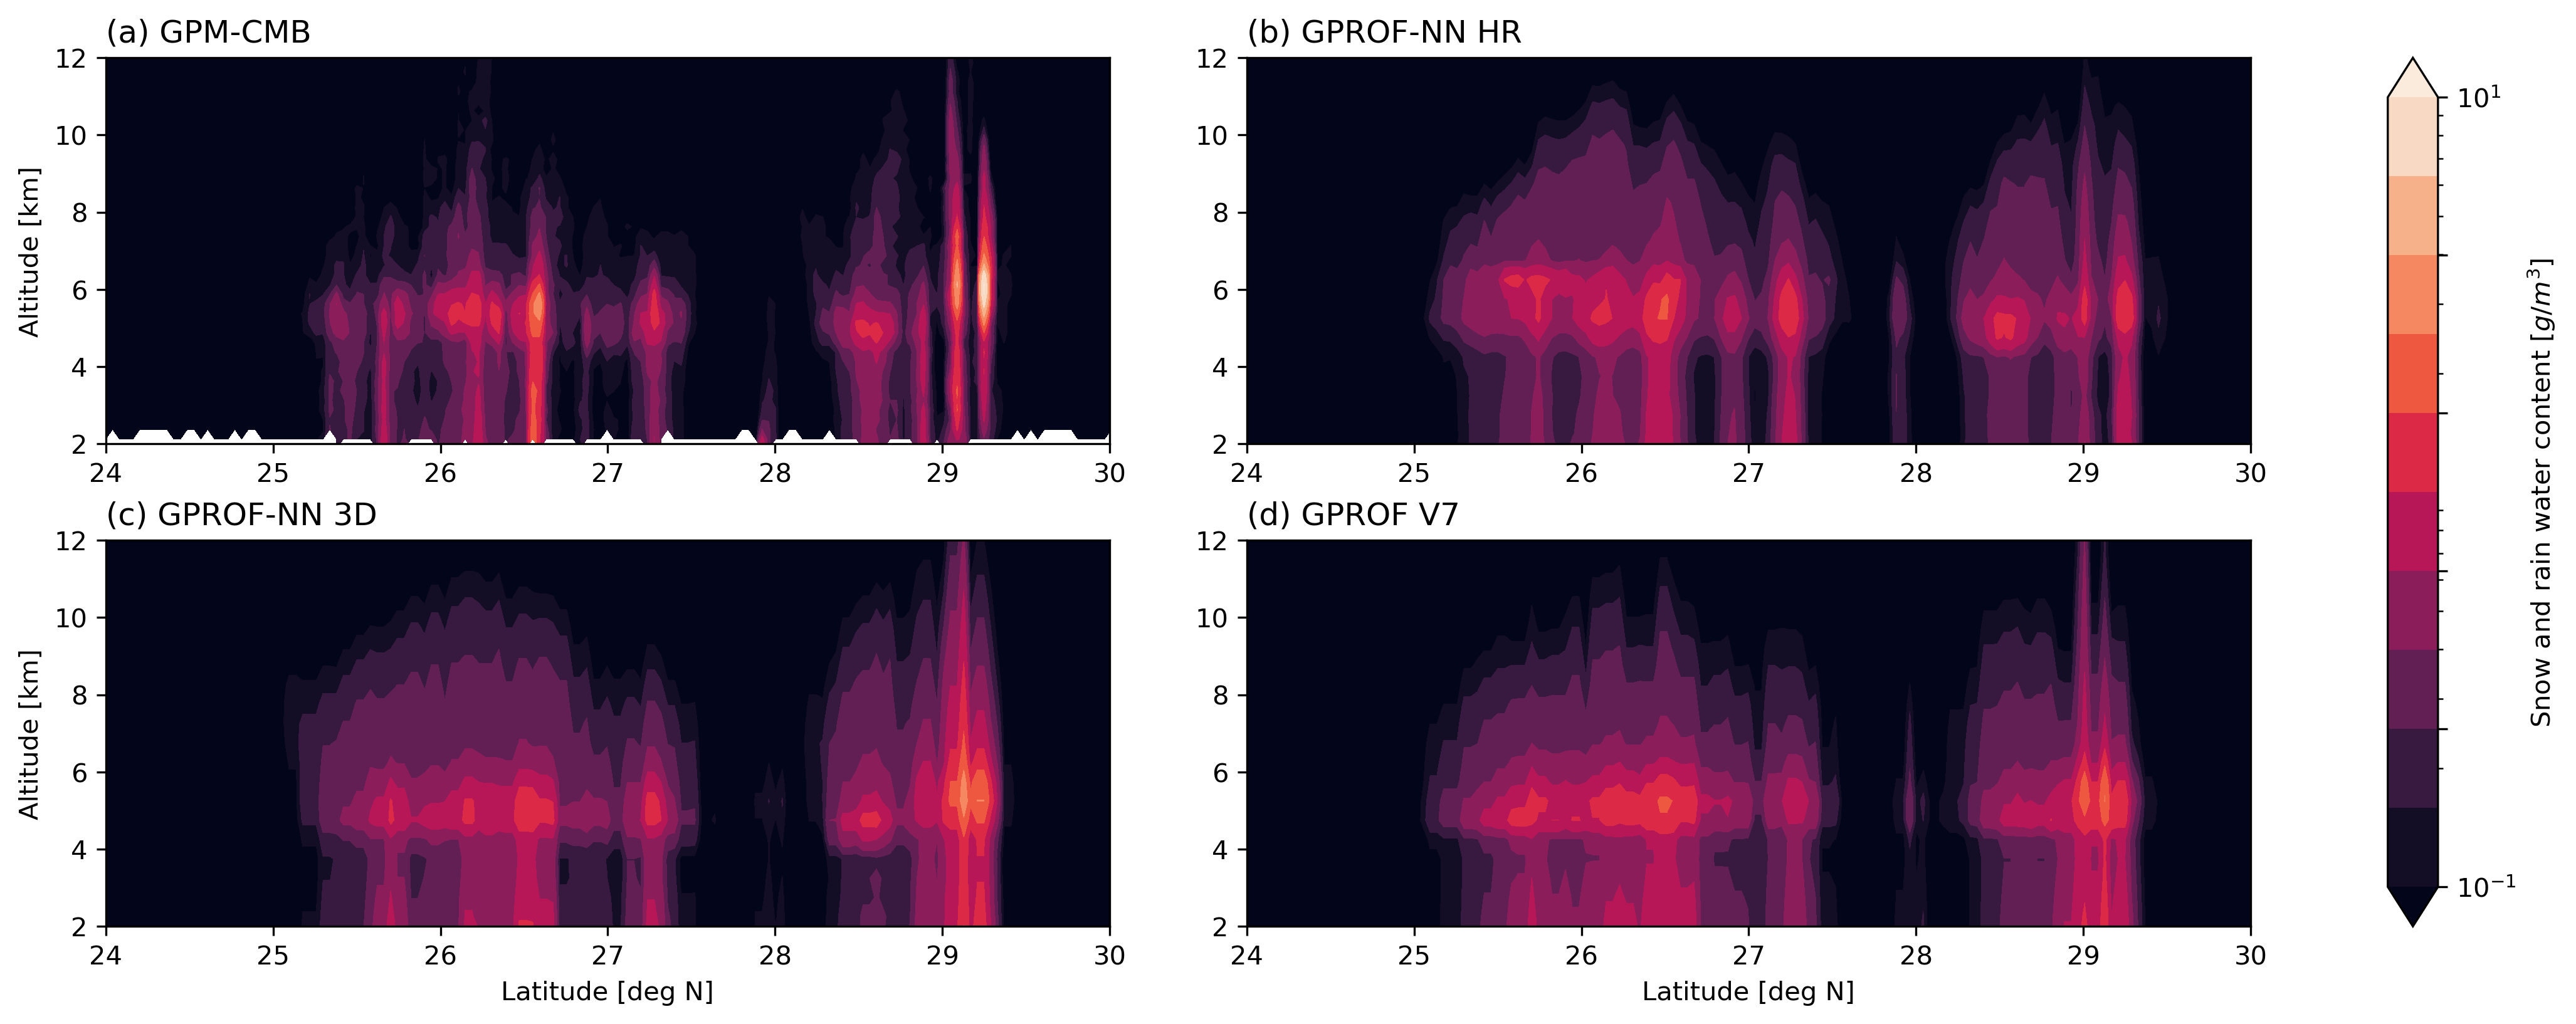
\includegraphics[width=\textwidth]{gprof_nn_hr}
%  \caption{Profiles of snow and rain water content in hurricane Ida. Each
%    panel shows retrieved precipitation profiles along the track of the
%    DPR on the GPM core observatory.
%  }
%  \label{fig:contributions:gprof_nn_hr}
%\end{figure}

\begin{figure}
  \centering
  \begin{subfigure}[b]{0.49\textwidth}
    \centering
    \includegraphics[width=\textwidth]{ida_gprof.0007}
    \caption{GPROF V7}
  \end{subfigure}
  \hfill
  \begin{subfigure}[b]{0.49\textwidth}
    \centering
    \includegraphics[width=\textwidth]{ida_gprof_nn_1d.0007}
    \caption{GPROF-NN 1D}
  \end{subfigure}
  \begin{subfigure}[b]{0.49\textwidth}
    \centering
    \includegraphics[width=\textwidth]{ida_gprof_nn_3d.0007}
    \caption{GPROF-NN 3D}
  \end{subfigure}
  \hfill
  \begin{subfigure}[b]{0.49\textwidth}
    \centering
    \includegraphics[width=\textwidth]{ida_gprof_hr.0007}
    \caption{GPROF-NN HR}
  \end{subfigure}
  \caption{
    Iso surfaces of rain water content (red) and snow water content (blue) in hurricane Ida
    shortly before landfall on 2021-08-29 15:14 UTC. For visualization purposes the
    vertical dimension is exaggerated by a factor of 10.
  }
  \label{fig:contributions:gprof_nn_hr}
\end{figure}


\subsection{Near real-time precipitation retrievals}

The results presented in \citet{pfreundschuh22b} clearly show the potential of
deep neural networks for precipitation retrievals from geostationary satellites.
According to personal communication, the developed retrieval is also being
considered for operational application.

An interesting result that emerged from this study was that, despite the low
information content of the geostationary observations on precipitation,
deep-learning-based retrievals can outperform highly complex retrieval pipelines
which integrate observations from multiple sensors. This indicates that the use
of information in current multi-sensor retrievals is sub-optimal. An upcoming
project will therefore explore the potential of directly fusing observations
from different sensors using a single neural network.
